\documentclass{article}

% if you need to pass options to natbib, use, e.g.:
%     \PassOptionsToPackage{numbers, compress}{natbib}
% before loading neurips_2021

% ready for submission
\usepackage[preprint]{neurips_2021}

% to compile a preprint version, e.g., for submission to arXiv, add add the
% [preprint] option:
%     \usepackage[preprint]{neurips_2021}

% to compile a camera-ready version, add the [final] option, e.g.:
%     \usepackage[final]{neurips_2021}

% to avoid loading the natbib package, add option nonatbib:
% \usepackage[nonatbib]{neurips_2021}
\usepackage[utf8]{inputenc} % allow utf-8 input
\usepackage[T1]{fontenc}    % use 8-bit T1 fonts
\usepackage[colorlinks = true, 
		    linkcolor = blue,
		    urlcolor  = blue,
            citecolor = blue,
            anchorcolor = blue]{hyperref}       
% hyperlinks
\usepackage{float}
\usepackage{url}            % simple URL typesetting
\usepackage{booktabs}       % professional-quality tables
\usepackage{amsfonts}       % blackboard math symbols
\usepackage{nicefrac}       % compact symbols for 1/2, etc.
\usepackage{microtype}      % microtypography
\usepackage{xcolor}         % colors
\usepackage{natbib}
\usepackage[pdftex]{graphicx}
\usepackage{siunitx} % Required for alignment
\sisetup{
  round-mode          = places, % Rounds numbers
  round-precision     = 2, % to 2 places
}
	
\bibliographystyle{unsrtnat}


\title{Extracting and evaluating educational concept dependencies from Large Language Models}

% The \author macro works with any number of authors. There are two commands
% used to separate the names and addresses of multiple authors: \And and \AND.
%
% Using \And between authors leaves it to LaTeX to determine where to break the
% lines. Using \AND forces a line break at that point. So, if LaTeX puts 3 of 4
% authors names on the first line, and the last on the second line, try using
% \AND instead of \And before the third author name.

\author{%
  Dominik Glandorf\\
  Matrikelnummer 6007407\\
  \texttt{dominik.glandorf@student.uni-tuebingen.de} \\
  \And
  Anastasiia Alekseeva\\
  Matrikelnummer 5994775\\
  \texttt{anastasiia.alekseeva@student.uni-tuebingen.de} \\
  \\
  GitHub repository: \url{https://github.com/mlcolab/learning-dependencies}
}

\begin{document}
\vspace*{-5mm}
\maketitle
\vspace*{-5mm}

\begin{abstract}
% What did we do?

% Why did we to it? What did we expect?

% How did we do it?

% What did we find out?

% What now?

\end{abstract}

\section{Introduction}
% Starting broad
% Field of contribution
Large Language Models (LLMs) are trained on immense corpora of text and have proven to build on embedded factual information when performing well in downstream tasks such as question answering. Accessing this knowledge, which is represented by billions of parameters and the network's architecture, has given rise to the research field of Knowledge Extraction from LLMs (\cite{cohen2023crawling}), which rests on the assumption that the language models can help retrieve information on the relation between entities. 

This work tries to contribute to the research field and to answer the question of whether general LLMs are able to provide a valid dependency structure of educational concepts. To find the answer to the research question, we are going to solve two main subtasks: 1) extraction of implicit educational concept dependencies, and 2) evaluation of the retrieved dependencies or the resulting graphs by existing knowledge media.

Apart from the field of knowledge extraction from LLMs, which is a subfield of computational linguistics, our work may contribute to applied education sciences by improving computer-assisted education and creating new perspectives for a subfield of knowledge engineering that has rather stagnated in the previous years.

% What kind of information do we want to extract?
%% Problem of sequencing in Instructional Design:
In particular, effective and efficient instruction does not only incorporate what to teach but also how to teach, especially the order of instruction.  It is proven that \textit{instructional sequencing} enhances the process of learning when prerequisites of educational content are known to the student or taught first \citep{morrison2019designing}.
% Definition concepts
Within educational content, Merill (1983) differentiated facts, concepts, principles, rules, procedures, interpersonal skills, attitudes, and their sole recall from their application. We will focus on concepts and their relations defined understanding. 
% Concept dependency
% Assumption: information about dependencies between concepts makes instructional sequencing more effective in terms of learning

To be more precise, if one concept is a prerequisite of another, we refer to this relation as a concept dependency. For example, to understand the concept of a derivative, having knowledge about the concept of a function will facilitate or even enable learning. When the dependencies are thought of as directed edges between nodes that represent concepts, a concept dependency graph emerges which is a special type of a knowledge graph \citep{wang2016using}. This graph is also called \textit{concept map} in the field of Learning Sciences.
% TODO: provide a (graphical) example of a small concept map
% Why is is important?
The graph can be used to advance curriculum planning (\cite{yang2015concept}), especially for new topics that might not be covered in textbooks or automated assessment (Wang, 2015).

% What is the gap in research that we tackle?
% What is our research question?
% How to extract educational concept dependencies that are implicit and evaluate them using existing knowledge media?
%In this work, we tackled the question how to extract this particular knowledge graph and how to evaluate its quality in a scalable manner.

% What can we contribute?
% 1. No benchmark available -> we set up an evaluation framework based on textbooks and Wikipedia
To conclude, our main contributions are the following.
First, there is little research on how to evaluate the precision of extracted concept dependencies. Therefore, we propose a set of methods to use existing unstructured knowledge sources, namely Wikipedia and textbooks, to create baselines for evaluation. Due to the heuristic character of these methods, we conducted a manual assessment to test their suitability for our purpose. The resulting dataset can be used as a baseline for further research.

% 2. Emerging field of prompt engineering -> we engineered a simple but effective prompt process to query a LLM
Second, the emerging field of prompt engineering provides a constellation of commands to query LLMs, the majority of which are experimental and cannot be considered fully reliable. We propose a method called \textit{output refeeding} that allows mining the educational concept dependencies by sequentially querying the language generation model and transforming its answers into a knowledge graph.

\subsection{Related work}
% Field: Concept Dependency Extraction
% of interest: How are concept dependencies defined?
\cite{talukdar2012crowdsourced} defined the prerequisite relation in terms of the consumption of information about concepts. Vuong (2011) if a better graduation rate given prerequisite knowledge is fulfilled. Concepts are often equated with Wikipedia articles (Talukdar and Cohen, 2012; Wang, 2015).

% Other approaches: Learning Path Analysis and Expert Knowledge
Prerequisites can be inferred from learner behavior by testing their performance after being presented different instructional sequences (Pavlik et al., 2008, Vuong et al., 2011). However, this has the disadvantage of disengaging users with too difficult concepts before teaching easier or necessary ones. Experts usually dispose of the required knowledge about concepts to create concept maps. The high cost of expert knowledge motivates the automated extraction of concept dependencies from appropriate sources.

% Field: Textbook Knowledge Extraction
% of interest: How are relationships betweens concepts extracted?

% Field: Prompt Engineering for Knowledge Graph creation
% of interest: How can we get internal representations out of a language model?
% Cohen, 2023 

Multiple approaches of prompt engineering for graph creation have been recently developed. Few-shot prompting proved successful (\cite{cohen2023crawling})

% GraphGPT

\section{Method}
% Section summary
In this section, we will first detail our research design and then the characteristics of our information sources as well as the methods that we used to produce the knowledge graph. 

\subsection{Research design} 

Our research lies at the intersection of education sciences and computational linguistics that define the choice of methodology. On the one hand, we prompt a state-of-the-art large language model to build entity dependency graphs and evaluate its performance on the concept relations retrieved from Wikipedia and textbooks. On the other hand, we should ensure that the output is sound in terms of educational value, which requires additional qualitative assessment.

Since no ground-truth knowledge graph exists and cannot be achieved in the field of education, we choose textbooks and Wikipedia as the baseline to be able to estimate the precision of the dependencies mined from the LLM. Each information extraction method is not fully independent of the other, in particular, entity recognition and concept disambiguation steps in the procedure for LLM and textbooks depend on Wikipedia. The evaluation was performed via 1) inspecting the output in the interactive dashboard, 2) manual labeling, and 3) convergence between the LLM and two baselines metric.

% two baseline methods: textbooks and Wikipedia
% information extraction: one LLM method
% evaluation
% 1. manual inspection via DashBoard
% 2. manual labeling
% 3. convergence between LLM and baselines

\subsection{Baseline extraction}
\subsubsection{Wikipedia}
% Why Wikipedia? % I asked ChatGPT :)

Wikipedia is a valuable resource that has a good structure of concepts. One of the key factors that contribute to it is the use of a hierarchical structure. Articles are categorized into broader topics, and those topics are further divided into subtopics. This structure helps readers to navigate through the information in a logical and organized manner, allowing them to quickly find the information they need. Another factor is the use of hyperlinks to connect related articles. This allows readers to move seamlessly between articles and explore related concepts without having to leave the site or perform additional searches. Wikipedia also has a strong editorial process that ensures that articles are well-researched, well-written, and up-to-date. This process helps to maintain the quality and accuracy of the information presented on the site, which in turn helps to reinforce the logical structure of the concepts presented.

% good coverage according to one of our papers
% 1462 unique articles for book index entries, these were covered in the textbooks (we had to select a subset of concepts to reduce computational effort)
% How did we get the information?
% describe Algorithm to extract dependencies:
%• Assumption: understanding the concept’s definition in Wikipedia requires understanding the concepts in it
%• Operationalization: links to other articles in the first sentence of article
%• Filtered out links to fields (“Mathematics”), persons (“Gabriel Cramer), and concepts that linked even earlier to the concept of interest

\subsubsection{Textbooks}
% Types of textbooks (why linear algebra?) % I asked ChatGPT :)

We chose textbooks on linear algebra as they tend to have a good structure and order compared to other textbooks because linear algebra is a well-established and mature field of mathematics with a clear and logical progression of concepts. Moreover, linear algebra is used extensively in other fields, such as engineering, physics, and computer science. Therefore, many textbooks on linear algebra are written with the needs of these fields in mind, which helps to structure the content of the textbook in a clear and practical manner. Finally, the concepts in linear algebra are interrelated, and a strong understanding of earlier topics is often necessary to understand later topics. 

We used 10 books that are free and available online. 
% Amount of data
% 10 books on Linear Algebra
% 584 pages on average (652,297 characters)
% 382 number of index entries (median)

% Steps of processing
% preprocessing
% entity recognition and disambigation
% Wikifier: identify entity mentions using link targets and PageRank
First, the textbooks were converted from pdf format to raw texts and went through basic preprocessing. Then, Wikifier \citep{brank2017annotating} was exploited for entity recognition and disambiguation.

% Wikisearch: query Wikipedia search engine for keyword (and field) and rank results based on Levenshtein distance

% relation extraction
% common introductory usage: identify other concepts that are most often mentioned on the first page given in the index across all books
% order pruning:  identify unlikely dependencies based on a certain number of books that introduce concepts in a particular order

\subsection{LLM extraction}
% description of T0PP and our infrastructure
% • Fine-tuned BLOOM on several question-answering datasets
% • 11 billion parameters (44GB RAM) • ~3-10 seconds per request on our infrastructure

% description of extraction procedure
% 1. output refeeding
% first prompt: {definition} := What is the mathematical definition of {concept}?
% second prompt:  {list of dependencies} := What mathematics concepts are mentioned here: {definition}
% 2. response parsing to Wikipedia article
% {canonical list of dependencies} :=Wikisearch disambiguation on {list of dependencies}

\begin{figure}
    \centering
    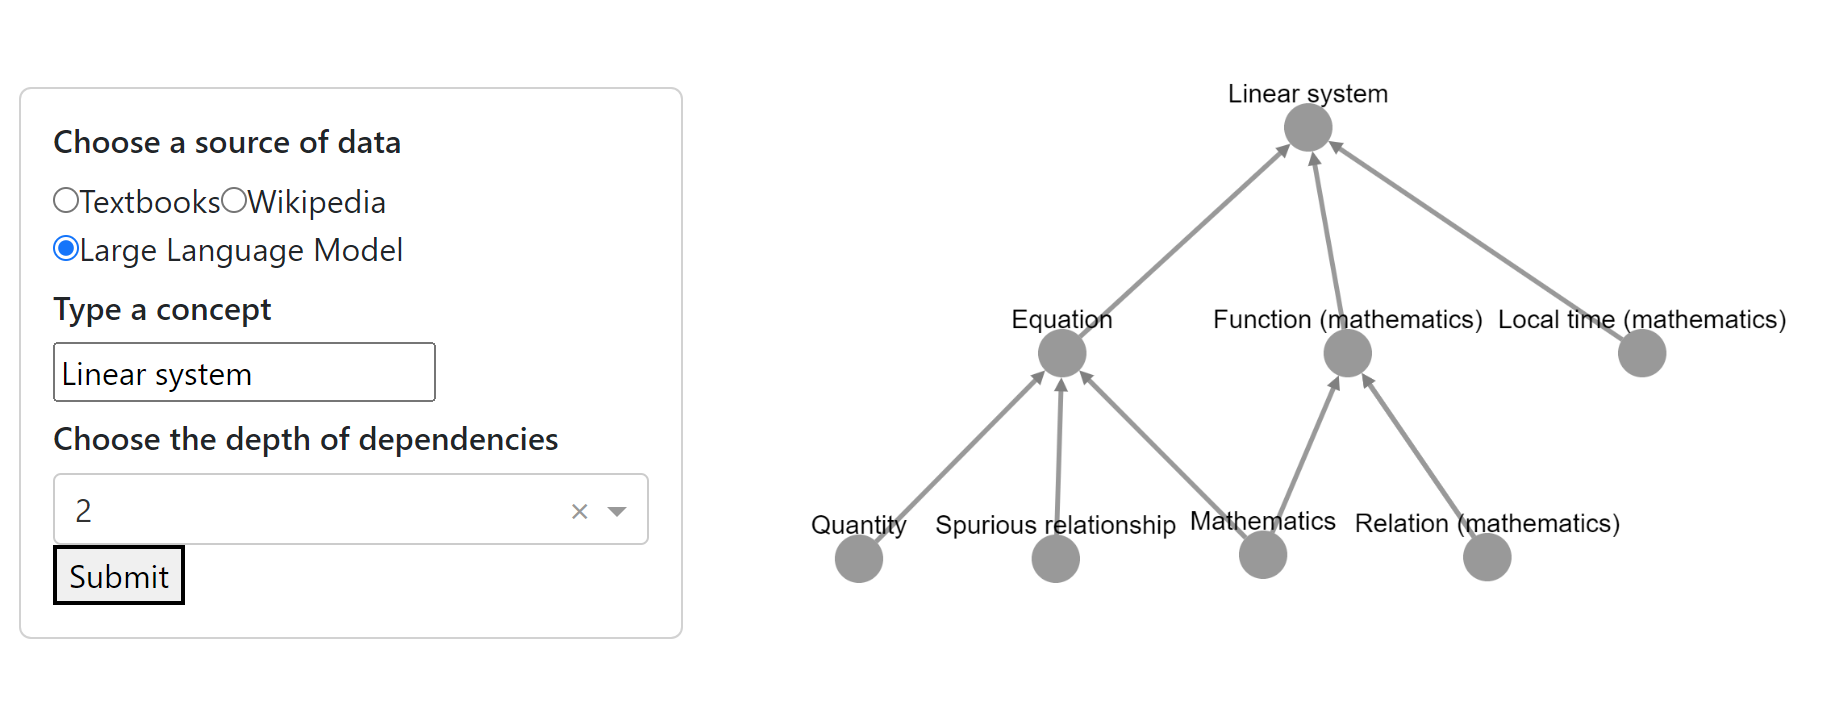
\includegraphics[width=.95\textwidth]{img/dash_example.png}
    \caption{A screenshot of the intercative application.}
    \label{fig:dash_example}
\end{figure}

\subsection{Manual inspection via Dashboard}
We developed a Dashboard via graphing library for Python Plotly\footnote{https://plotly.com/python/} (Fig.\ref{fig:dash_example}). The application is devised so that one could examine the resulting graph itself in a convenient environment. It allows plotting the concept dependencies graphs for three knowledge sources or types of dependency mining methods (LLM, Wikipedia, and textbooks) for different levels of dependencies.   



\subsection{Manual baseline}
% procedure to assess the accuracy of output

\subsection{Convergence statistics}
% for which concepts did we compare what to see what

\section{Results}
% Case Study using Dashboard

%Manual baseline
% Interrater reliability
% How good are the baselines?
% How good is the LLM?
% diagram


\begin{figure}[H]
    \centering
    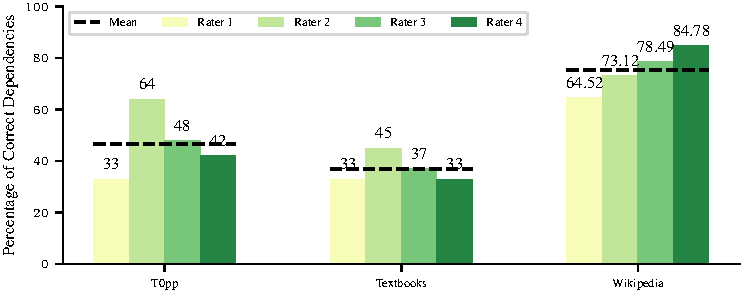
\includegraphics[width=.95\textwidth]{img/rating.pdf}
    \caption{Rating.}
    \label{fig:rating}
\end{figure}

\begin{figure}[H]
    \centering
    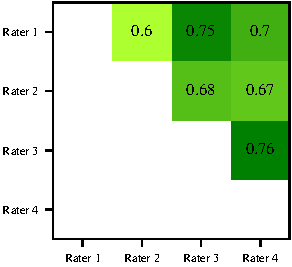
\includegraphics[width=.4\textwidth]{img/kappa.pdf}
    \caption{Interrater reliability, kappa coefficient.}
    \label{fig:kappa}
\end{figure}

%Convergence statistics
% diagram for similarity of outputs

\begin{figure}
    \centering
    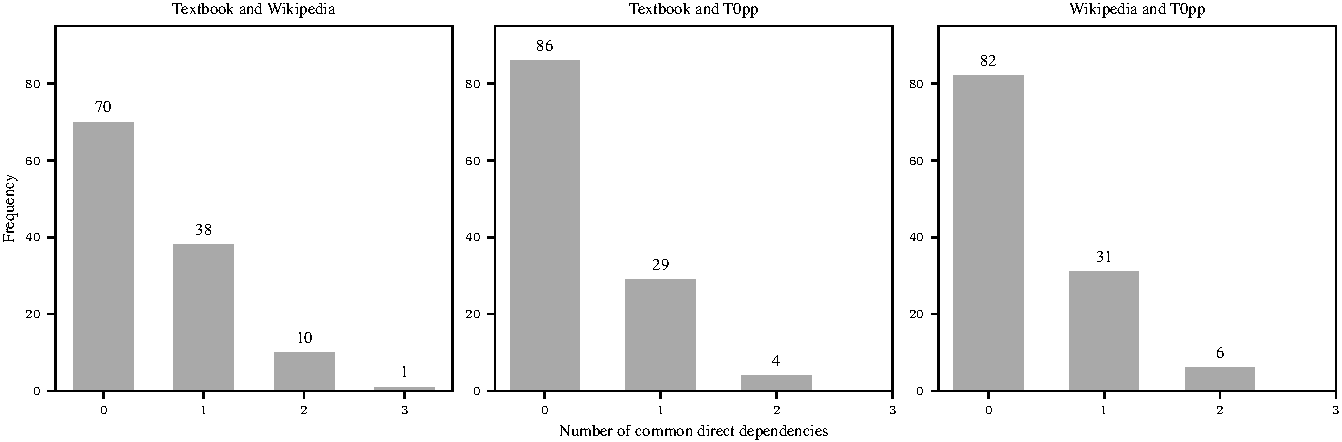
\includegraphics[width=.95\textwidth]{img/comp_direct_deps.pdf}
    \caption{Convergence metrics. Number of common direct dependencies between sources.}
    \label{fig:comp_direct_deps}
\end{figure}

\section{Discussion}
% What is our main result?
% we are able to make the implicit knowledge explicit far above chance level
% problem is very complex -> humans do not fully agree
% Wikipedia might be the best source to automatically evaluate the output

% What are potential flaws?

% disambiguation already includes noise
% error propagation

% we only evaluated up to two levels of the graph, not the graph as a whole. different level of abstractions in extracted dependencies
% is there even something like a gold standard? some educational reflection about different didactic approaches and more depth than just understanding the definition of a topic
% Cohen et al (2023) think that there is no gold standard, ground truth.

% we are still using the language generator, so it is just another downstream task, maybe it is more of a philosophical question what is implicit/explicit knowledge


% + "I don't know" option in the prompt engineering part
% + Google search

% Q: Outlook and Future research ideas:

As shown, current LLMs are not sufficiently precise in creating concept maps, which confirms previous research \cite{hwang2021comet}. This could be improved by training the pre-trained models on the knowledge graph data mined from Wikipedia or any other reliable sources of concept dependencies in a specific subject of instruction \cite{west2022symbolic}.
% advancements in LLMs that are interesting for us
% use cases in education


\bibliography{references.bib}

\newpage


\section{Appendix}



\begin{figure}[H]
    \centering
    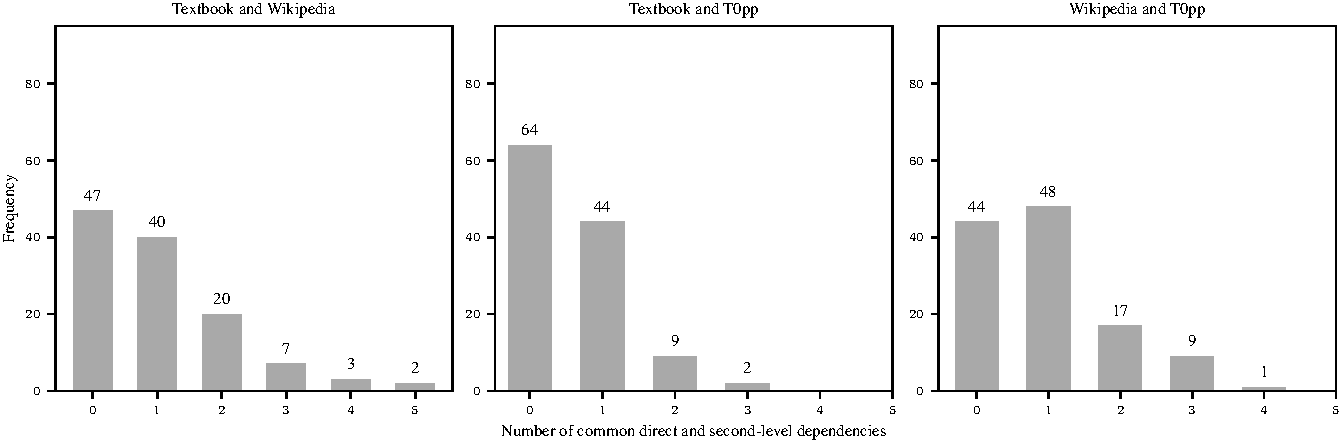
\includegraphics[width=.95\textwidth]{img/comp_second_deps.pdf}
    \caption{Convergence metrics. Number of common direct and second-level dependencies between sources.}
    \label{fig:comp_second_deps}
\end{figure}






\end{document}
